%% LyX 2.3.6.2 created this file.  For more info, see http://www.lyx.org/.
%% Do not edit unless you really know what you are doing.
\documentclass[english,aspectratio=169,handout]{beamer}
\usepackage{mathptmx}
\usepackage{eulervm}
\usepackage[T1]{fontenc}
\usepackage[latin9]{inputenc}
\usepackage{babel}
\usepackage{amstext}
\usepackage{amssymb}
\usepackage{graphicx}
\usepackage{comment}
\ifx\hypersetup\undefined
  \AtBeginDocument{%
    \hypersetup{unicode=true,pdfusetitle,
 bookmarks=true,bookmarksnumbered=false,bookmarksopen=false,
 breaklinks=false,pdfborder={0 0 0},pdfborderstyle={},backref=false,colorlinks=true,
 allcolors=NYUPurple,urlcolor=LightPurple}
  }
\else
  \hypersetup{unicode=true,pdfusetitle,
 bookmarks=true,bookmarksnumbered=false,bookmarksopen=false,
 breaklinks=false,pdfborder={0 0 0},pdfborderstyle={},backref=false,colorlinks=true,
 allcolors=NYUPurple,urlcolor=LightPurple}
\fi

\makeatletter


%%%%%%%%%%%%%%%%%%%%%%%%%%%%%% LyX specific LaTeX commands.
%% Because html converters don't know tabularnewline
\providecommand{\tabularnewline}{\\}

%%%%%%%%%%%%%%%%%%%%%%%%%%%%%% Textclass specific LaTeX commands.
% this default might be overridden by plain title style
\newcommand\makebeamertitle{\frame{\maketitle}}%
% (ERT) argument for the TOC
\AtBeginDocument{%
  \let\origtableofcontents=\tableofcontents
  \def\tableofcontents{\@ifnextchar[{\origtableofcontents}{\gobbletableofcontents}}
  \def\gobbletableofcontents#1{\origtableofcontents}
}

%%%%%%%%%%%%%%%%%%%%%%%%%%%%%% User specified LaTeX commands.
\usetheme{CambridgeUS} 
\beamertemplatenavigationsymbolsempty


% Set Color ==============================
\definecolor{NYUPurple}{RGB}{87,6,140}
\definecolor{LightPurple}{RGB}{165,11,255}


\setbeamercolor{title}{fg=NYUPurple}
%\setbeamercolor{frametitle}{fg=NYUPurple}
\setbeamercolor{frametitle}{fg=NYUPurple}

\setbeamercolor{background canvas}{fg=NYUPurple, bg=white}
\setbeamercolor{background}{fg=black, bg=NYUPurple}

\setbeamercolor{palette primary}{fg=black, bg=gray!30!white}
\setbeamercolor{palette secondary}{fg=black, bg=gray!20!white}
\setbeamercolor{palette tertiary}{fg=gray!20!white, bg=NYUPurple}

\setbeamertemplate{headline}{}

\setbeamercolor{parttitle}{fg=NYUPurple}
\setbeamercolor{sectiontitle}{fg=NYUPurple}
\setbeamercolor{sectionname}{fg=NYUPurple}
\setbeamercolor{section page}{fg=NYUPurple}

\AtBeginSection[]{
  \begin{frame}
    \frametitle{Table of Contents}
    \tableofcontents[currentsection]
  \end{frame}

  % \begin{frame}
  % \vfill
  % \centering
  % \begin{beamercolorbox}[sep=8pt,center,shadow=true,rounded=true]{title}
  %   \usebeamerfont{title}\insertsectionhead\par%
  % \end{beamercolorbox}
  % \vfill
  % \end{frame}
}

\makeatother

\begin{document}
\global\long\def\reals{\mathbf{R}}%
 
\global\long\def\integers{\mathbf{Z}}%
 
\global\long\def\naturals{\mathbf{N}}%
 
\global\long\def\rationals{\mathbf{Q}}%
 
\global\long\def\ca{\mathcal{A}}%
 
\global\long\def\cb{\mathcal{B}}%
 
\global\long\def\cc{\mathcal{C}}%
 
\global\long\def\cd{\mathcal{D}}%
 
\global\long\def\ce{\mathcal{E}}%
 
\global\long\def\cf{\mathcal{F}}%
 
\global\long\def\cg{\mathcal{G}}%
 
\global\long\def\ch{\mathcal{H}}%
 
\global\long\def\ci{\mathcal{I}}%
 
\global\long\def\cj{\mathcal{J}}%
 
\global\long\def\ck{\mathcal{K}}%
 
\global\long\def\cl{\mathcal{L}}%
 
\global\long\def\cm{\mathcal{M}}%
 
\global\long\def\cn{\mathcal{N}}%
 
\global\long\def\co{\mathcal{O}}%
 
\global\long\def\cp{\mathcal{P}}%
 
\global\long\def\cq{\mathcal{Q}}%
 
\global\long\def\calr{\mathcal{R}}%
 
\global\long\def\cs{\mathcal{S}}%
 
\global\long\def\ct{\mathcal{T}}%
 
\global\long\def\cu{\mathcal{U}}%
 
\global\long\def\cv{\mathcal{V}}%
 
\global\long\def\cw{\mathcal{W}}%
 
\global\long\def\cx{\mathcal{X}}%
 
\global\long\def\cy{\mathcal{Y}}%
 
\global\long\def\cz{\mathcal{Z}}%
 
\global\long\def\ind#1{1(#1)}%
 %\newcommand{\pr}{P}
\global\long\def\pr{\mathbb{P}}%
 
\global\long\def\predsp{\cy}%
 %{\hat{\cy}}
\global\long\def\outsp{\cy}%

\global\long\def\prxy{P_{\cx\times\cy}}%
 
\global\long\def\prx{P_{\cx}}%
 
\global\long\def\prygivenx{P_{\cy\mid\cx}}%
 %\newcommand{\ex}{E}
\global\long\def\ex{\mathbb{E}}%
 
\global\long\def\var{\textrm{Var}}%
 
\global\long\def\cov{\textrm{Cov}}%
 
\global\long\def\sgn{\textrm{sgn}}%
 
\global\long\def\sign{\textrm{sign}}%
 
\global\long\def\kl{\textrm{KL}}%
 
\global\long\def\law{\mathcal{L}}%
 
\global\long\def\eps{\varepsilon}%
 
\global\long\def\as{\textrm{ a.s.}}%
 
\global\long\def\io{\textrm{ i.o.}}%
 
\global\long\def\ev{\textrm{ ev.}}%
 
\global\long\def\convd{\stackrel{d}{\to}}%
 
\global\long\def\eqd{\stackrel{d}{=}}%
 
\global\long\def\del{\nabla}%
 
\global\long\def\loss{\ell}%
 
\global\long\def\risk{R}%
 
\global\long\def\emprisk{\hat{R}}%
 
\global\long\def\lossfnl{L}%
 
\global\long\def\emplossfnl{\hat{L}}%
 
\global\long\def\empminimizer#1{\hat{#1}^{*}}%
 
\global\long\def\minimizer#1{#1^{*}}%
\global\long\def\optimizer#1{#1^{*}}%
 
\global\long\def\etal{\textrm{et. al.}}%
 
\global\long\def\tr{\operatorname{tr}}%

\global\long\def\trace{\operatorname{trace}}%
 
\global\long\def\diag{\text{diag}}%
 
\global\long\def\rank{\text{rank}}%
 
\global\long\def\linspan{\text{span}}%
 
\global\long\def\spn{\text{span}}%
 
\global\long\def\proj{\text{Proj}}%
 
\global\long\def\argmax{\operatornamewithlimits{arg\, max}}%
 
\global\long\def\argmin{\operatornamewithlimits{arg\, min}}%

\global\long\def\bfx{\mathbf{x}}%
 
\global\long\def\bfy{\mathbf{y}}%
 
\global\long\def\bfl{\mathbf{\lambda}}%
 
\global\long\def\bfm{\mathbf{\mu}}%
 
\global\long\def\calL{\mathcal{L}}%

\global\long\def\vw{\boldsymbol{w}}%
 
\global\long\def\vx{\boldsymbol{x}}%
 
\global\long\def\vxi{\boldsymbol{\xi}}%
 
\global\long\def\valpha{\boldsymbol{\alpha}}%
 
\global\long\def\vbeta{\boldsymbol{\beta}}%
 
\global\long\def\vsigma{\boldsymbol{\sigma}}%
\global\long\def\vtheta{\boldsymbol{\theta}}%
 
\global\long\def\vd{\boldsymbol{d}}%
 
\global\long\def\vs{\boldsymbol{s}}%
 
\global\long\def\vt{\boldsymbol{t}}%
 
\global\long\def\vh{\boldsymbol{h}}%
 
\global\long\def\ve{\boldsymbol{e}}%
 
\global\long\def\vf{\boldsymbol{f}}%
 
\global\long\def\vg{\boldsymbol{g}}%
 
\global\long\def\vz{\boldsymbol{z}}%
 
\global\long\def\vk{\boldsymbol{k}}%
 
\global\long\def\va{\boldsymbol{a}}%
 
\global\long\def\vb{\boldsymbol{b}}%
 
\global\long\def\vv{\boldsymbol{v}}%
 
\global\long\def\vy{\boldsymbol{y}}%

\global\long\def\dom{\textrm{\textbf{dom} }}%
\global\long\def\rank{\text{\textbf{rank }}}%
\global\long\def\conv{\textrm{\textbf{conv} }}%
\global\long\def\relint{\text{\textbf{relint }}}%
\global\long\def\aff{\text{\textbf{aff }}}%

\global\long\def\hil{\ch}%
 
\global\long\def\rkhs{\hil}%
 
\global\long\def\ber{\text{Ber}}%

\global\long\def\softmax{\text{Softmax}}%

\title[DS-GA 1003 ]{Probabilistic models\\
- \\
Bayesian Methods}
% \author{Tal Linzen \\
% Slides based on Lecture
% \href{https://github.com/davidrosenberg/mlcourse/blob/gh-pages/Lectures/08a.bayesian-methods.pdf}{08a} from David Rosenberg's course materials (\url{https://github.com/davidrosenberg/mlcourse}) and Marylou Gabri\'e's materials
% }
\date{March 21, 2023}
\institute{CDS, NYU}

% \title[DS-GA 1003]{Bayesian Methods}
% \author{Julia Kempe \& David S. Rosenberg }
% \date{March 26, 2019}
% \institute{CDS, NYU}

\makebeamertitle
\mode<article>{Just in article version}

\begin{frame}{Contents}

\tableofcontents{}
\end{frame}

\section{Classical Statistics}
\begin{frame}{Parametric Family of Densities}
\begin{itemize}
\item A \textbf{parametric family of densities }is a set 
\[
\left\{ p(y\mid\theta):\theta\in\Theta\right\} ,
\]

\begin{itemize}
\item where $p(y\mid\theta)$ is a density on a \textbf{sample space }$\cy$,
and
\item $\theta$ is a \textbf{parameter} in a {[}finite dimensional{]} \textbf{parameter
space $\Theta$.}
\end{itemize}
\end{itemize}

\pause{}
\begin{itemize}
\item This is the common starting point for a treatment of classical or
Bayesian statistics.
\item In this lecture, whenever we say ``density'', we could replace it
    with ``mass function.'' (and replace integrals with sums).{\scriptsize{} }{\scriptsize\par}
\end{itemize}
\end{frame}

\begin{frame}{Frequentist or ``Classical'' Statistics}
\begin{itemize}
\item We're still working with a parametric family of densities:
\[
\left\{ p(y\mid\theta)\mid\theta\in\Theta\right\} .
\]
\end{itemize}

\pause{}
\begin{itemize}
\item Assume that $p(y\mid\theta)$ governs the world we are observing,
for some $\theta\in\Theta$.
\end{itemize}

\pause{}
\begin{itemize}
\item If we knew the right $\theta\in\Theta$, there would be no need for
statistics.
\end{itemize}

\pause{}
\begin{itemize}
\item But instead of $\theta$, we have data $\cd$: $y_{1},\ldots,y_{n}$ sampled
i.i.d. from $p(y\mid\theta)$.
\end{itemize}

\pause{}
\begin{itemize}
\item Statistics is about how to get by with $\cd$ in place of $\theta$.
\end{itemize}
\end{frame}
%

\begin{frame}{Point Estimation}

\begin{itemize}
\item One type of statistical problem is\textbf{ point estimation}.
\end{itemize}

\pause{}
\begin{itemize}
\item A \textbf{statistic} $s=s(\cd)$ is any function of the data.
\end{itemize}

\pause{}
\begin{itemize}
\item A statistic $\hat{\theta}=\hat{\theta}(\cd)$ taking values in $\Theta$
is a\textbf{ point estimator of} $\theta$.
\end{itemize}

\pause{}
\begin{itemize}
\item A good point estimator will have $\hat{\theta}\approx\theta$.
% \end{itemize}
% \end{frame}
% %
% \begin{frame}{Desirable Properties of Point Estimators}
% \begin{itemize}
\item \textbf{Desirable statistical properties of point estimators}:

\pause{}
\begin{itemize}
\item \textbf{Consistency: }As data size $n\to\infty$, we get $\hat{\theta}_{n}\to\theta$.
\end{itemize}

\pause{}
\begin{itemize}
\item \textbf{Efficiency:} (Roughly speaking) $\hat{\theta}_{n}$ is as
accurate as we can get from a sample of size $n$.
\end{itemize}
\end{itemize}

\pause{}
\begin{itemize}
\item \textbf{Maximum likelihood estimators }are consistent and efficient
under reasonable conditions.
\end{itemize}
\end{frame}
%
% \begin{frame}{The Likelihood Function}
% \begin{itemize}
% \item Consider parametric family $\left\{ p(y\mid\theta):\theta\in\Theta\right\} $
% and i.i.d. sample $\cd=\left(y_{1},\ldots,y_{n}\right)$.

% \pause{}
% \item The density for sample $\cd$ for $\theta\in\Theta$ is
% \[
% p(\cd\mid\theta)\pause=\prod_{i=1}^{n}p(y_{i}\mid\theta).
% \]


% \pause{}
% \item $p(\cd\mid\theta)$ is a function of $\cd$ and $\theta$. 

% \pause{}
% \item For fixed $\theta$, $p(\cd\mid\theta$) is a density function on
% $\cy^{n}$.

% \pause{}
% \item For fixed $\cd$, the function $\theta\mapsto p(\cd\mid\theta)$ is
% called the \textbf{likelihood function:
% \[
% L_{\cd}(\theta):=p(\cd\mid\theta).
% \]
% }
% \end{itemize}
% \end{frame}
% %
% \begin{frame}{Maximum Likelihood Estimation}
% \begin{definition}
% The \textbf{maximum likelihood estimator (MLE)} for $\theta$ in the
% model $\left\{ p(y\mid\theta):\theta\in\Theta\right\} $ is
% \begin{eqnarray*}
% \hat{\theta}_{\text{MLE}} & = & \argmax_{\theta\in\Theta}L_{\cd}(\theta).
% \end{eqnarray*}

% \pause{}
% \end{definition}

% \begin{itemize}
% \item Maximum likelihood is just one approach to getting a point estimator
% for $\theta$.

% \pause{}
% \item \textbf{Method of moments} is another general approach one learns
% about in statistics.

% \pause{}
% \item Later we'll talk about \textbf{MAP }and \textbf{posterior mean }as
% approaches to point estimation.
% \begin{itemize}
% \item These arise naturally in Bayesian settings.
% \end{itemize}
% \end{itemize}
% \end{frame}
%
\begin{frame}{Example of Point Estimation: Coin Flipping}
\begin{itemize}
\item Parametric family of mass functions:
\[
p(\text{Heads}\mid\theta)=\theta,
\]
for $\theta\in\Theta=\left(0,1\right)$.
\end{itemize}
\end{frame}
%
\begin{frame}{Coin Flipping: MLE}
\begin{itemize}
\item Data $\cd=\left(H,H,T,T,T,T,T,H,\ldots,T\right)$, assumed i.i.d. flips.
\begin{itemize}
\item $n_{h}$: number of heads
\item $n_{t}$: number of tails\textbf{ }
\end{itemize}
% \item 

\pause{}
\item \textbf{Likelihood function }for data $\cd$:

\[
L_{\cd}(\theta)=\pause p(\cd\mid\theta)=\theta^{n_{h}}\left(1-\theta\right)^{n_{t}}
\]

% \pause{}
% \item (This is the probability of getting the flips in the order they were
% received)
% \end{itemize}
% \end{frame}
%
% \begin{frame}{Coin Flipping: MLE}
 
% \begin{itemize}
\item As usual, it is easier to maximize the log-likelihood function:
\begin{eqnarray*}
\hat{\theta}_{\text{MLE}} & = & \argmax_{\theta\in\Theta}\log L_{\cd}(\theta)\\
 & = & \argmax_{\theta\in\Theta}\left[n_{h}\log\theta+n_{t}\log(1-\theta)\right]
\end{eqnarray*}
\end{itemize}

\pause{}
\begin{itemize}
    \item First order condition (equating the derivative to zero):
\[
\frac{n_{h}}{\theta}-\frac{n_{t}}{1-\theta} = 0 \iff\theta  =  \frac{n_{h}}{n_{h}+n_{t}} \pause \quad \quad  \hat{\theta}_{\text{MLE}} \text{ is the empirical fraction of heads.}
\]
% \item So $\hat{\theta}_{\text{MLE}}$ 
\end{itemize}
\end{frame}

\section{Bayesian Statistics: Introduction}
\begin{frame}{Bayesian Statistics}
 

\begin{itemize}
\item Baysian statistics introduces a crucial new ingredient: the \textbf{prior distribution.}
\end{itemize}

\pause{}
\begin{itemize}
\item A \textbf{prior distribution} $p(\theta)$ is a distribution on the parameter
space $\Theta$.
\end{itemize}

\pause{}
\begin{itemize}
\item The prior reflects our belief about $\theta$, \textbf{before seeing
any data}.
\end{itemize}
\end{frame}
%
\begin{frame}{A Bayesian Model }
\begin{itemize}
\item A {[}parametric{]} Bayesian model consists of two pieces:
\begin{enumerate}
\item A parametric family of densities 
\[
\left\{ p(\cd\mid\theta)\mid\theta\in\Theta\right\} .
\]


\pause{}
\item A \textbf{prior distribution} $p(\theta)$ on parameter space $\Theta$.

\pause{}
\end{enumerate}
\item Putting the pieces together, we get a joint density on $\theta$ and $\cd$:
\[
p(\cd,\theta)=p(\cd\mid\theta)p(\theta).
\]
\end{itemize}
\end{frame}
%
\begin{frame}{The Posterior Distribution}
\begin{itemize}
\item The \textbf{posterior distribution }for $\theta$ is $p(\theta\mid\cd)$.
\end{itemize}

\pause{}
\begin{itemize}
\item Whereas the prior represents belief about $\theta$ before observing data $\cd$,
\end{itemize}

\pause{}
\begin{itemize}
\item The posterior represents the\textbf{ rationally updated belief}
about $\theta$, after seeing $\cd$.
\end{itemize}
\end{frame}
%
\begin{frame}{Expressing the Posterior Distribution}
\begin{itemize}
\item By Bayes rule, can write the posterior distribution as
\[
p(\theta\mid\cd)\pause=\frac{p(\cd\mid\theta)p(\theta)}{p(\cd)}.
\]


\pause{}
\item Let's consider both sides as functions of $\theta$, for fixed $\cd$.

\pause{}
\item Then both sides are densities on $\Theta$ and we can write
\[
\underbrace{p(\theta\mid\cd)}_{\text{posterior}}\propto\underbrace{p(\cd\mid\theta)}_{\text{likelihood}}\underbrace{p(\theta)}_{\text{prior}}.
\]


\pause{}
\item Where $\propto$ means we've dropped factors that are independent of $\theta$. 
\end{itemize}
\end{frame}
%
\begin{frame}{Coin Flipping: Bayesian Model}
\begin{itemize}
\item Recall that we have a parametric family of mass functions:
\[
p(\text{Heads}\mid\theta)=\theta,
\]
for $\theta\in\Theta=\left(0,1\right)$.
\end{itemize}

\pause{}
\begin{itemize}
\item We need a prior distribution $p(\theta)$ on $\Theta=(0,1)$.
\end{itemize}

\pause{}
\begin{itemize}
\item One convenient choice would be a distribution from the Beta family
\end{itemize}
\end{frame}
%
\begin{frame}{Coin Flipping: Beta Prior}
\begin{itemize}
\item \textbf{Prior:}
\begin{eqnarray*}
\theta & \sim & \text{Beta}(\alpha,\beta)\\
p(\theta) & \propto & \theta^{\alpha-1}\left(1-\theta\right)^{\beta-1}
\end{eqnarray*}


\pause{}
\end{itemize}
\begin{center}
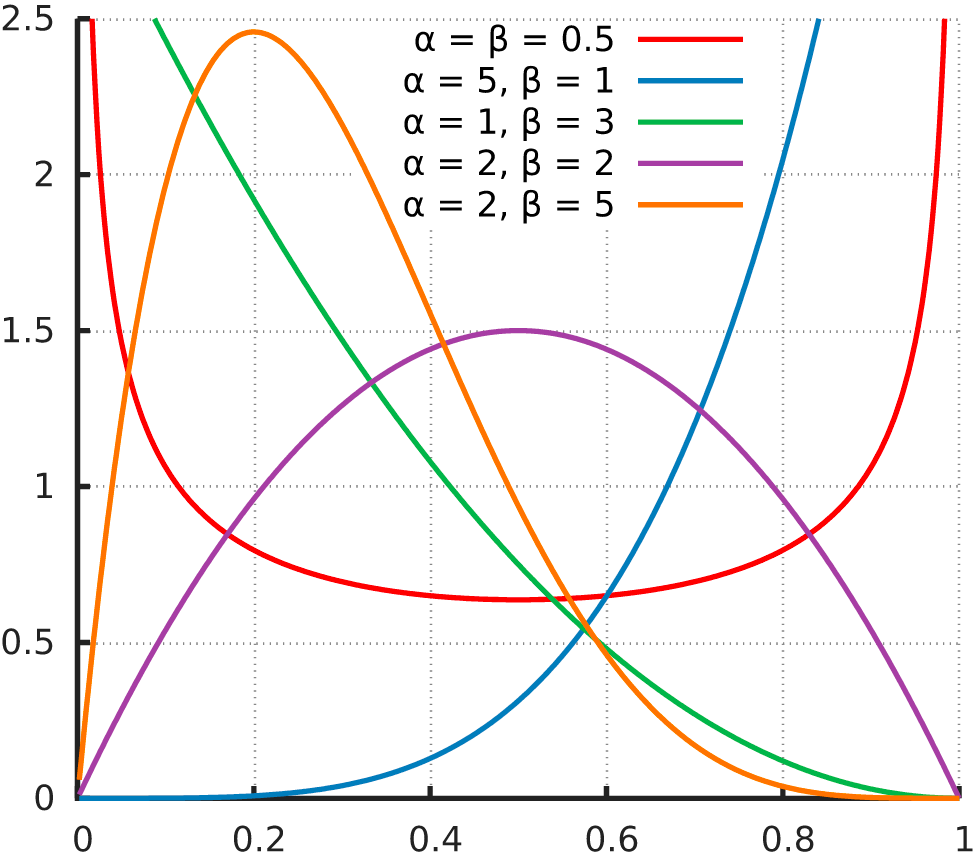
\includegraphics[height=0.55\textheight]{figs/betaFamily}
\par\end{center}

\let\thefootnote\relax\footnotetext{\tiny{Figure by Horas based on the work of Krishnavedala (Own work) [Public domain], via Wikimedia Commons \url{http://commons.wikimedia.org/wiki/File:Beta_distribution_pdf.svg}.}}
\end{frame}
%
\begin{frame}{Coin Flipping: Beta Prior}
\begin{itemize}
\item \textbf{Prior:}
\begin{eqnarray*}
\theta & \sim & \text{Beta}(h,t)\\
p(\theta) & \propto & \theta^{h-1}\left(1-\theta\right)^{t-1}
\end{eqnarray*}


\pause{}
\item \textbf{Mean of Beta distribution:} 
\[
\ex\theta=\frac{h}{h+t}
\]


\pause{}
\item \textbf{Mode of Beta distribution:} 
\[
\argmax_{\theta}p(\theta)=\frac{h-1}{h+t-2}
\]
for $h,t>1$.
\end{itemize}
\end{frame}
%
\begin{frame}{Coin Flipping: Posterior}
\begin{itemize}
\item \textbf{Prior:}
\begin{eqnarray*}
\theta & \sim & \text{Beta}(h,t)\\
p(\theta) & \propto & \theta^{h-1}\left(1-\theta\right)^{t-1}
\end{eqnarray*}
\end{itemize}

\pause{}
\begin{itemize}
\item \textbf{Likelihood function}
\[
L(\theta)=p(\cd\mid\theta)=\theta^{n_{h}}\left(1-\theta\right)^{n_{t}}
\]
\end{itemize}

\pause{}
\begin{itemize}
\item \textbf{Posterior density:}
\begin{eqnarray*}
p(\theta\mid\cd) & \propto & p(\theta)p(\cd\mid\theta)\\
\pause & \propto & \theta^{h-1}\left(1-\theta\right)^{t-1}\times\theta^{n_{h}}\left(1-\theta\right)^{n_{t}}\\
\pause & = & \theta^{h-1+n_{h}}\left(1-\theta\right)^{t-1+n_{t}}
\end{eqnarray*}
 
\end{itemize}
\end{frame}
%
\begin{frame}{The Posterior is in the Beta Family!}
\begin{itemize}
\item \textbf{Prior:}
\begin{eqnarray*}
\theta & \sim & \text{Beta}(h,t)\\
p(\theta) & \propto & \theta^{h-1}\left(1-\theta\right)^{t-1}
\end{eqnarray*}
 
\item \textbf{Posterior density:}
\begin{eqnarray*}
p(\theta\mid\cd) & \propto & \theta^{h-1+n_{h}}\left(1-\theta\right)^{t-1+n_{t}}
\end{eqnarray*}
\end{itemize}

\pause{}
\begin{itemize}
\item \textbf{Posterior is in the beta family}:
\begin{eqnarray*}
\theta\mid\cd & \sim & \text{Beta}(h+n_{h},t+n_{t})
\end{eqnarray*}
\end{itemize}

\pause{}
\begin{itemize}
\item \textbf{Interpretation}:
\begin{itemize}
\item Prior initializes our counts with $h$ heads and $t$ tails.
\item Posterior increments counts by observed $n_{h}$ and $n_{t}$. 
\end{itemize}
\end{itemize}
\end{frame}
%
\begin{frame}{Sidebar: Conjugate Priors}
\begin{itemize}
\item In this case, the posterior is in the same distribution family as the prior.
\item Let $\pi$ be a family of prior distributions on $\Theta$.

\pause{}
\item Let $P$ parametric family of distributions with parameter space $\Theta$.

\pause{}

\end{itemize}
\begin{definition}
A family of distributions \textbf{$\pi$ is conjugate to }parametric
model \textbf{$P$} if for any prior in $\pi$, the posterior is always
in $\pi$.

\pause{}
\end{definition}

\begin{itemize}
\item The beta family is conjugate to the coin-flipping (i.e. Bernoulli)
model.

%\pause{}
%\item The family of all probability distributions is conjugate to any parametric
%model. {[}Trvially{]}
\end{itemize}

\end{frame}
%
\begin{frame}{Coin Flipping: Concrete Example}
\begin{itemize}
\item Suppose we have a coin, possibly biased (\textbf{parametric probability
model}):
\[
p(\mbox{Heads}\mid\theta)=\theta.
\]


\pause{}
\item \textbf{Parameter space }$\theta\in\Theta=[0,1]$. 
\item \textbf{Prior distribution: }$\theta\sim\mbox{Beta}(2,2)$.

\pause{}
\end{itemize}
\begin{center}
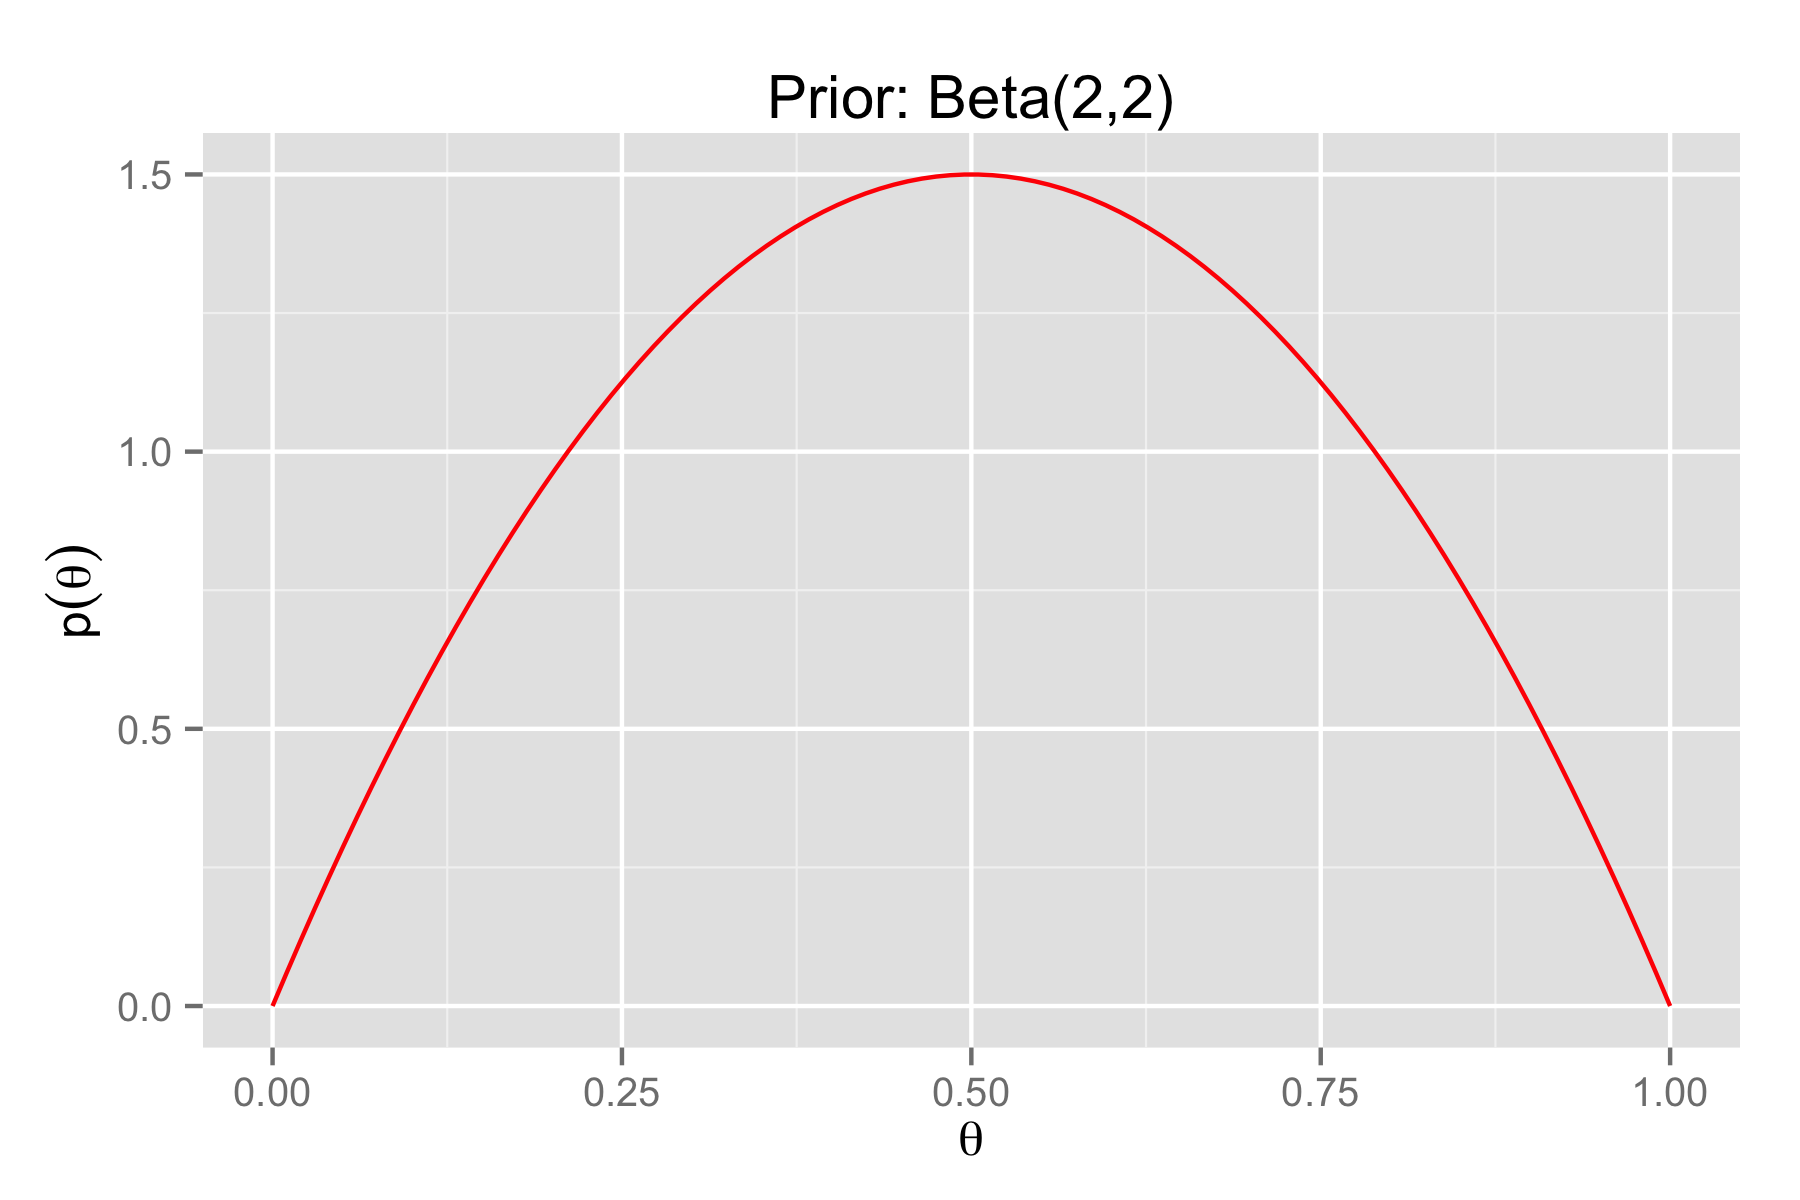
\includegraphics[height=0.5\textheight]{figs/beta2-2}
\par\end{center}

\end{frame}
%
\begin{frame}{Example: Coin Flipping}
\begin{itemize}
\item Next, we gather some data $\cd=\left\{ H,H,T,T,T,T,T,H,\ldots,T\right\} $:
\end{itemize}

\pause{}
\begin{itemize}
\item Heads: 75\qquad{}Tails: 60 

\pause{}
\begin{itemize}
\item $\hat{\theta}_{\text{MLE}}=\frac{75}{75+60}\approx0.556$

\pause{}
\end{itemize}
\item \textbf{Posterior distribution: $\theta\mid\cd\sim\mbox{Beta}(77,62)$:}
\end{itemize}
\begin{center}
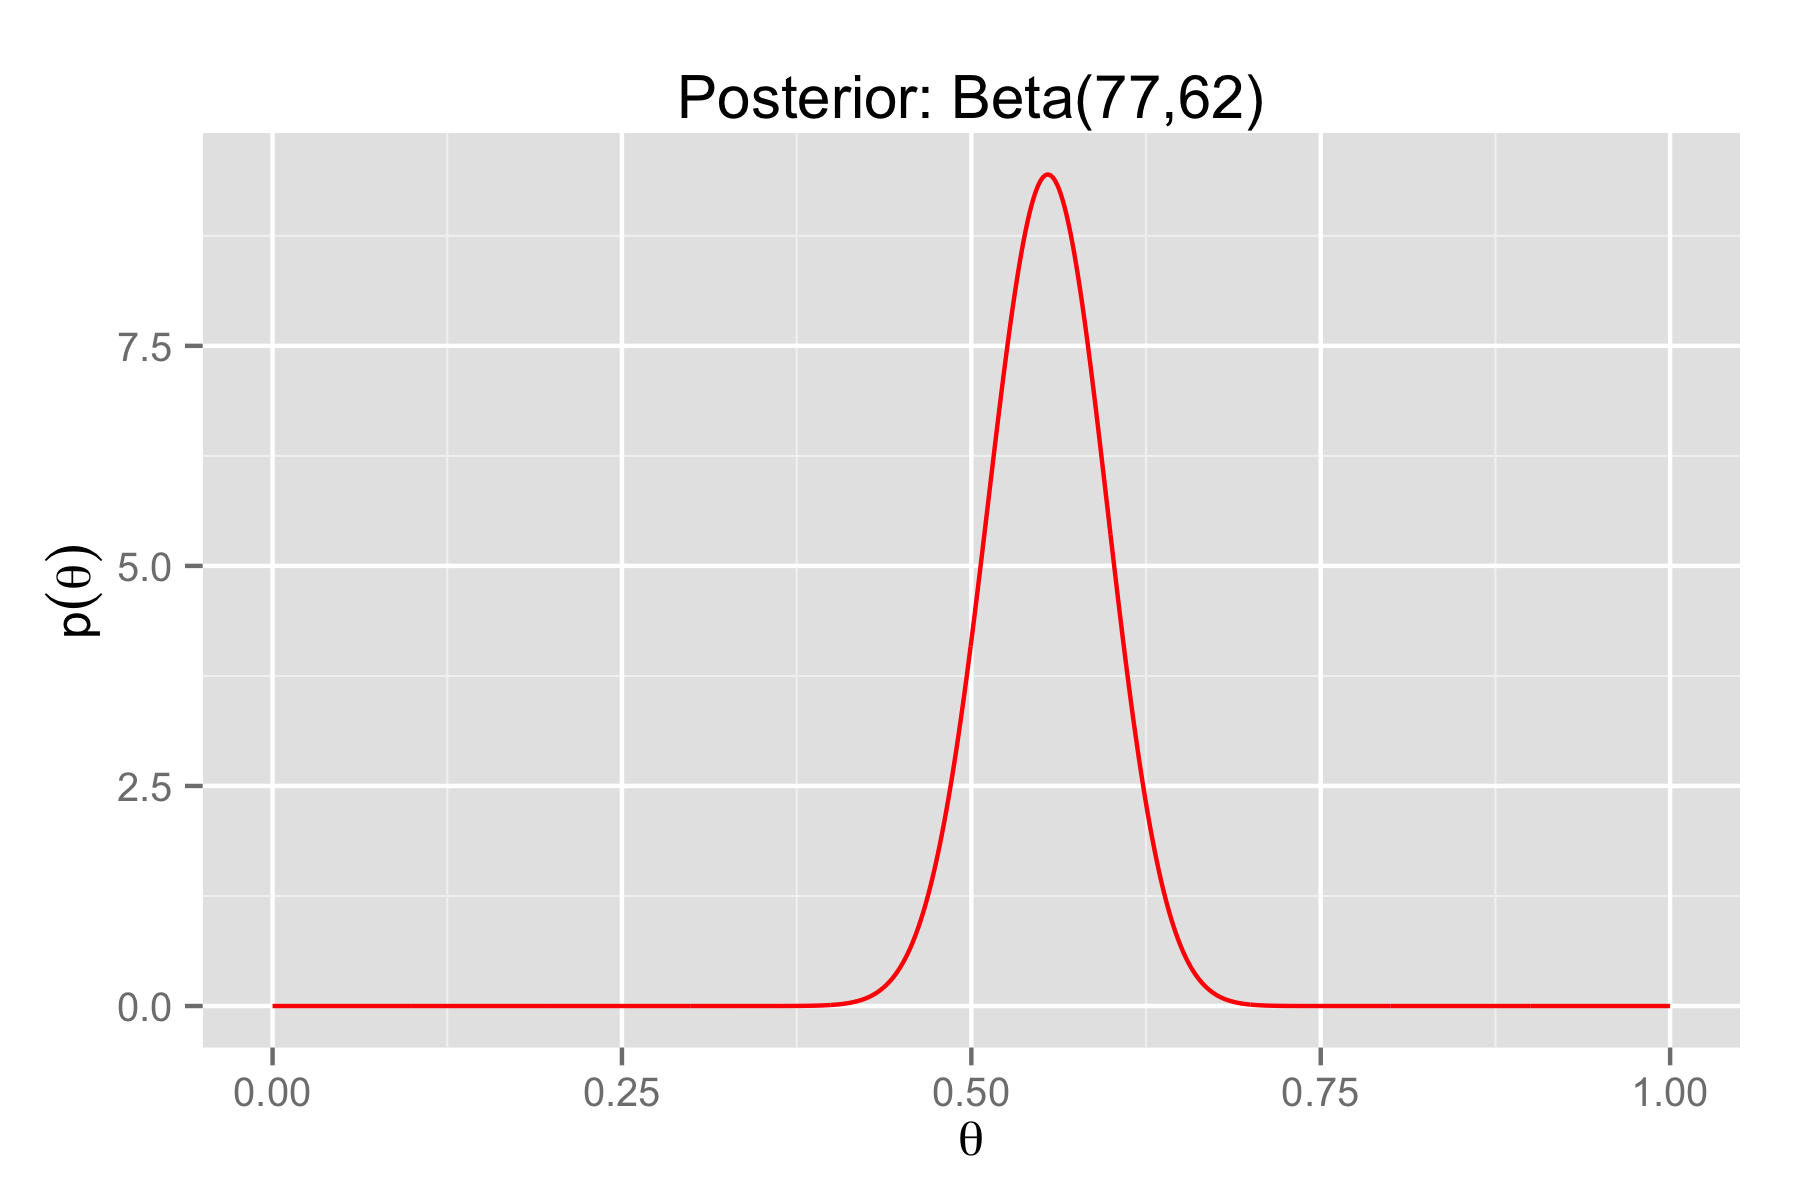
\includegraphics[height=0.6\textheight]{figs/beta77-62}
\par\end{center}

\end{frame}

\begin{frame}{Bayesian Point Estimates}
\begin{itemize}
\item We have the posterior distribution $\theta\mid\cd$.
\item What if someone asks us for a point estimate $\hat{\theta}$ for $\theta$?

\pause{}
\item Common options:

\pause{}
\begin{itemize}
\item \textbf{posterior mean} $\hat{\theta}=\ex\left[\theta\mid\cd\right]$

\pause{}
\item \textbf{maximum a posteriori (MAP) estimate} $\hat{\theta}=\argmax_{\theta}p(\theta\mid\cd)$ 
\begin{itemize}
\item Note: this is the \textbf{mode} of the posterior distribution
\end{itemize}
\end{itemize}
\end{itemize}
\end{frame}
%
\begin{frame}{What else can we do with a posterior?}
\begin{itemize}
\item Look at it: display uncertainty estimates to our client

\pause{}
\item Extract a \textbf{credible set} for $\theta$ (a Bayesian confidence
interval).
\begin{itemize}
\item e.g. Interval $[a,b]$ is a $95\%$\textbf{ credible set} if\textbf{
\[
\pr\left(\theta\in[a,b]\mid\cd\right)\ge0.95
\]
 }
\end{itemize}

\pause{}
\item Select a point estimate using \textbf{Bayesian decision theory}:
\begin{itemize}
\item Choose a loss function.
\item Find action \textbf{minimizing expected risk w.r.t. posterior}
\end{itemize}
\end{itemize}

\end{frame}

\section{Bayesian Decision Theory}
\begin{frame}{Bayesian Decision Theory}
\begin{itemize}
\item Ingredients: 
\begin{itemize}
\item \textbf{Parameter space} $\Theta$.
\item \textbf{Prior}: Distribution $p(\theta)$ on $\Theta$.
\item \textbf{Action space} $\ca$.
\item \textbf{Loss function}: $\ell:\ca\times\Theta\to\reals$.

\pause{}
\end{itemize}
\item The \textbf{posterior risk} of an action $a\in\ca$ is 
\begin{eqnarray*}
r(a) & := & \ex\left[\ell(\theta,a)\mid\cd\right]\\
\pause & = & \int\ell(\theta,a)p(\theta\mid\cd)\,d\theta.
\end{eqnarray*}


\pause{}
\begin{itemize}
\item It's the \textbf{expected loss under the posterior.}

\pause{}
\end{itemize}
\item A \textbf{Bayes action} $a^{*}$ is an action that minimizes posterior
risk:
\[
r(a^{*})=\min_{a\in\ca}r(a)
\]
\end{itemize}
\end{frame}
%
\begin{frame}{Bayesian Point Estimation}
\begin{itemize}
\item General Setup:
\begin{itemize}
\item Data $\cd$ generated by $p(y\mid\theta)$, for unknown $\theta\in\Theta$.

\pause{}
\item We want to produce a \textbf{point estimate} for $\theta$.

\pause{}
\end{itemize}
\item Choose:

\pause{}
\begin{itemize}
\item \textbf{Prior} $p(\theta)$ on $\Theta=\reals$.

\pause{}
\item \textbf{Loss} $\ell(\hat{\theta},\theta)$ %=\left(\theta-\hat{\theta}\right)^{2}$ 

\pause{}
\end{itemize}
\item Find \textbf{action} $\hat{\theta}\in\Theta$ that minimizes the \textbf{
posterior risk:}
\begin{eqnarray*}
r(\hat{\theta}) & = & \ex\left[\ell(\hat{\theta},\theta)\mid\cd\right]\\
\pause & = & \int\ell(\hat{\theta},\theta)p(\theta\mid\cd)\,d\theta
\end{eqnarray*}
\end{itemize}
\end{frame}
%
\begin{frame}{Important Cases}
\begin{itemize}
  \item Squared Loss :  $\ell(\hat{\theta},\theta)=\left(\theta-\hat{\theta}\right)^{2} \quad \Rightarrow$ posterior mean
  \item Zero-one Loss:  $\ell(\theta,\hat{\theta})=\ind{\theta\neq\hat{\theta}}\quad \Rightarrow $ posterior mode
  \item Absolute Loss :  $\ell(\hat{\theta},\theta)=\left|\theta-\hat{\theta}\right| \quad \Rightarrow$ posterior median
\end{itemize}
\end{frame}
%
\begin{frame}{Bayesian Point Estimation: Square Loss}
\begin{itemize}
\item Find \textbf{action} $\hat{\theta}\in\Theta$ that minimizes\textbf{
posterior risk} 
\begin{eqnarray*}
r(\hat{\theta}) & = & \int\left(\theta-\hat{\theta}\right)^{2}p(\theta\mid\cd)\,d\theta.
\end{eqnarray*}


\pause{}
\item Differentiate:
\end{itemize}
\begin{eqnarray*}
\frac{dr(\hat{\theta})}{d\hat{\theta}} & = & -\int2\left(\theta-\hat{\theta}\right)p(\theta\mid\cd)\,d\theta\\
\pause & = & -2\int\theta p(\theta\mid\cd)\,d\theta+2\hat{\theta}\underbrace{\int p(\theta\mid\cd)\,d\theta}_{=1}\\
\pause & = & -2\int\theta p(\theta\mid\cd)\,d\theta+2\hat{\theta}
\end{eqnarray*}

\end{frame}
%
\begin{frame}{Bayesian Point Estimation: Square Loss}
\begin{itemize}
\item Derivative of posterior risk is
\[
\frac{dr(\hat{\theta})}{d\hat{\theta}}=-2\int\theta p(\theta\mid\cd)\,d\theta+2\hat{\theta}.
\]


\pause{}
\item First order condition $\frac{dr(\hat{\theta})}{d\hat{\theta}}=0$
gives
\begin{eqnarray*}
\hat{\theta} & = & \int\theta p(\theta\mid\cd)\,d\theta\\
\pause & = & \ex\left[\theta\mid\cd\right]
\end{eqnarray*}
\end{itemize}

\pause{}
\begin{itemize}
\item The \textbf{Bayes action }for \textbf{square loss} is the posterior mean.
\end{itemize}
\end{frame}
%
% \begin{frame}{Bayesian Point Estimation: Absolute Loss}
% \begin{itemize}
% \item \textbf{Loss:}\emph{ $\ell(\theta,\hat{\theta})=\left|\theta-\hat{\theta}\right|$}

% \pause{}
% \item \textbf{Bayes action} for \textbf{absolute loss} is the \textbf{posterior
% median.}
% \begin{itemize}
% \item That is, the median of the distribution $p(\theta\mid\cd)$.

% \pause{}
% \item Show with approach similar to what was used in Homework \#1.
% \end{itemize}
% \end{itemize}
% \end{frame}
%
%\begin{frame}{Bayesian Point Estimation: Zero-One Loss}
%\begin{itemize}
%\item Suppose $\Theta$ is discrete (e.g. $\Theta=\left\{ \mbox{english},\mbox{french}\right\} $)
%\item \textbf{Zero-one loss:}\emph{ $\ell(\theta,\hat{\theta})=\ind{\theta\neq\hat{\theta}}$}

%\pause{}
%\item \textbf{Posterior risk}:
%\begin{eqnarray*}
%r(\hat{\theta}) & = & \ex\left[\ind{\theta\neq\hat{\theta}}\mid\cd\right]\\
%\pause & = & \pr\left(\theta\neq\hat{\theta}\mid\cd\right)\\
%\pause & = & 1-\pr\left(\theta=\hat{\theta}\mid\cd\right)\\
%\pause & = & 1-p(\hat{\theta}\mid\cd)
%\end{eqnarray*}


%\pause{}
%\item \textbf{Bayes action} is
%\begin{eqnarray*}
%\hat{\theta} & = & \argmax_{\theta\in\Theta}p(\theta\mid\cd)
%\end{eqnarray*}


%\pause{}
%\item This $\hat{\theta}$ is called the\textbf{ maximum a posteriori (MAP)
%}estimate.
%\item The MAP estimate is the \textbf{mode} of the posterior distribution.
%\end{itemize}
%\end{frame}

\section{Interim summary}
\begin{frame}{Recap and Interpretation}
\begin{itemize}
\item The prior represents belief about $\theta$ before observing data $\cd$.
\item The posterior represents \textbf{ rationally updated beliefs}
after seeing $\cd$.

\pause{}
\item All inferences and action-taking are based on the posterior distribution.

\pause{}
\item In the Bayesian approach,
\begin{itemize}
\item No issue of justifying an estimator.

\pause{}
\item Only choices are
\begin{itemize}
\item \textbf{family of distributions}, indexed by $\Theta$, and
\item \textbf{prior distribution }on $\Theta$

\pause{}
\end{itemize}
\item For decision making, we need a \textbf{loss function}.
\end{itemize}
\end{itemize}
\emph{}
\end{frame}
%
%\begin{frame}{The Bayesian Method}
 
%\begin{enumerate}
%\item \textbf{Define the model}:
%\begin{itemize}
%\item Choose a parametric family of densities: 
%\[
%\left\{ p(\cd\mid\theta)\mid\theta\in\Theta\right\} .
%\]
 
%\item Choose a distribution $p(\theta)$ on $\Theta$, called the \textbf{prior
%distribution}.

%\pause{}
%\end{itemize}
%\item After observing $\cd$, compute the \textbf{posterior distribution}
%$p(\theta\mid\cd)$. 

%\pause{}
%\item Choose  \textbf{action} based on $p(\theta\mid\cd)$. 
%\end{enumerate}
%\end{frame}
%

\section{Recap: Conditional Probability Models}
\begin{frame}{Conditional Probability Modeling}

\begin{itemize}
\item \textbf{Input space} $\cx$
\item \textbf{Outcome space} $\cy$ 

% \pause{}
\item \textbf{Action space} $\ca=\left\{ p(y)\mid p\text{ is a probability distribution on }\cy\right\} $.

\pause{}
\item \textbf{Hypothesis space} $\cf$ contains prediction functions $f:\cx\to\ca$. 

% \pause{}
\item \textbf{Prediction function} $f\in\cf$ takes input $x\in\cx$ and
produces a \textbf{distribution} on $\cy$

\pause{}
% \item We've been discussing \textbf{parametric families of conditional densities}
% \[
% \left\{ p(y\mid x,\theta):\theta\in\Theta\right\} .
% \]


% \pause{}
% \item These are also hypothesis spaces for conditional probability modeling.

% \pause{}
% \item Examples?
% \end{itemize}
% \end{frame}
% %
% \begin{frame}{Parametric Family of Conditional Densities}
% \begin{itemize}
\item A \textbf{parametric family of conditional densities }is a set 
\[
\left\{ p(y\mid x,\theta):\theta\in\Theta\right\} ,
\]

\begin{itemize}
\item where $p(y\mid x,\theta)$ is a density on \textbf{outcome space }$\cy$
for each $x$ in \textbf{input space $\cx$}, and
\item $\theta$ is a \textbf{parameter} in a {[}finite dimensional{]} \textbf{parameter
space $\Theta$.}
\end{itemize}
\end{itemize}

\pause{}
\begin{itemize}
\item This is the common starting point for either classical or
Bayesian regression.
\end{itemize}
\end{frame}
%
% \begin{frame}{Density vs Mass Functions}
% \begin{itemize}
% \item In this lecture, whenever we say ``density'', we could replace it
% with ``mass function.'' 
% \end{itemize}

% \pause{}
% \begin{itemize}
% \item Corresponding integrals would be replaced by summations.{\scriptsize{} }{\scriptsize\par}
% \end{itemize}

% \pause{}
% \begin{itemize}
% \item {\small{}(In more advanced, measure-theoretic treatments, they are
% each considered densities w.r.t. different base measures.)}{\small\par}
% \end{itemize}
% \end{frame}
%
% \begin{frame}{The Data: Assumptions So Far in this Course}
% \begin{itemize}
% \item Our usual setup is that $(x,y)$ pairs are drawn i.i.d. from $\cp_{\cx\times\cy}$.

% \pause{}
% \item How have we used this assumption so far?

% \pause{}
% \begin{itemize}
% \item ties validation performance to test performance
% \item ties test performance to performance on new data when deployed
% \item motivates empirical risk minimization

% \pause{}
% \end{itemize}
% \item The large majority of things we've learned about ridge/lasso/elastic-net
% regression, optimization, SVMs, and kernel methods are true for arbitrary
% training data sets $\cd:\left(x_{1},y_{1}\right),\ldots,\left(x_{n},y_{n}\right)\in\cx\times\cy$.
% \begin{itemize}
% \item i.e. $\cd$ could be created by hand, by an adversary, or randomly.

% \pause{}
% \end{itemize}
% \item We rely on the i.i.d. $\cp_{\cx\times\cy}$ assumption when it comes
% to \textbf{generalization}.
% \end{itemize}
% \end{frame}
% %
% \begin{frame}{The Data: Conditional Probability Modeling}
% \begin{itemize}
% \item To get generalization, we'll still need our usual i.i.d. $\cp_{\cx\times\cy}$
% assumption.
% \end{itemize}

% \pause{}
% \begin{itemize}
% \item For developing the model, we'll make some assumptions about the training
% data...
% \begin{itemize}
% \item In most of what we've done before, we had no assumptions on the training
% data.
% \end{itemize}
% \end{itemize}

% \pause{}
% \begin{itemize}
% \item It's typical (and most general) to do everything ``conditional on
% the $x$'s''
% \begin{itemize}
% \item That means, we assume the $x$'s are known

% \pause{}
% \item In particular, we do not consider them random

% \pause{}
% \item We don't care how they were generated (randomly, adversarially, chosen
% by hand) 

% \pause{}
% \item In other words, still no assumptions on $x$'s. 
% \end{itemize}
% \end{itemize}
% \end{frame}
% %
% \begin{frame}{The Data: Conditional Probability Modeling}
% \begin{itemize}
% \item So we assume the $x$'s are known.
% \end{itemize}

% \pause{}
% \begin{itemize}
% \item We observe $y_{i}$ sampled randomly from $p(y\mid x_{i},\theta)$,
% for some unknown $\theta\in\Theta$. 
% \end{itemize}

% \pause{}
% \begin{itemize}
% \item We assume the outcomes $y_{1},\ldots,y_{n}$ are independent. 
% \begin{itemize}
% \item But not i.i.d. -- Why?
% \end{itemize}

% \pause{}
% \begin{itemize}
% \item Each $y_{i}$ may be drawn from a different distribution, depending
% on $x_{i}$.
% \end{itemize}

% \end{itemize}
% \end{frame}
%
\begin{frame}{Classical treatment: Likelihood Function}
\begin{itemize}
\item \textbf{Data: }$\cd=(y_{1},\ldots,,y_{n})$
\item The probability density for our data $\cd$ is
\begin{eqnarray*}
p(\cd\mid x_{1},\ldots,x_{n},\theta) & = & \prod_{i=1}^{n}p(y_{i}\mid x_{i},\theta).
\end{eqnarray*}


\pause{}
\item For fixed $\cd$, the function $\theta\mapsto p(\cd\mid x,\theta)$
is the \textbf{likelihood function}:
\[
L_{\cd}(\theta)=p(\cd\mid x,\theta),
\]
where $x=\left(x_{1},\ldots,x_{n}\right)$.
\end{itemize}
\end{frame}
%
\begin{frame}{Maximum Likelihood Estimator}
\begin{itemize}
\item The \textbf{maximum likelihood estimator (MLE)} for $\theta$ in the
family $\left\{ p(y\mid x,\theta)\mid\theta\in\Theta\right\} $ is
\begin{eqnarray*}
\hat{\theta}_{\text{MLE}} & = & \argmax_{\theta\in\Theta}L_{\cd}(\theta).
\end{eqnarray*}


% \pause{}
\item MLE corresponds to ERM, if we set the loss to be the negative log-likelihood.

\pause{}
\item The corresponding prediction function is
\[
\hat{f}(x)=p(y\mid x,\hat{\theta}_{\text{MLE}}).
\]


%\pause{}
%\item We can think of this as a choice of a particular function from the
%hypothesis space
%\[
%\cf=\left\{ p(y\mid x,\theta):\theta\in\Theta\right\} .
%\]
\end{itemize}
\end{frame}

\section{Bayesian Conditional Probability Models}
\begin{frame}{Bayesian Conditional Models}
\begin{itemize}
\item Input space $\cx=\reals^{d}$\qquad{}Outcome space $\cy=\reals$
\end{itemize}

\pause{}
\begin{itemize}
\item The Bayesian conditional model has two components:
\begin{itemize}
\item A \textbf{parametric family of conditional densities}: 
\[
\left\{ p(y\mid x,\theta):\theta\in\Theta\right\} 
\]
\end{itemize}

\pause{}
\begin{itemize}
\item A \textbf{prior distribution} $p(\theta)$ on $\theta\in\Theta$. 
\end{itemize}
\end{itemize}
\end{frame}
%
\begin{frame}{The Posterior Distribution}
\begin{itemize}
\item The \textbf{prior distribution} $p(\theta)$ represents our beliefs
about $\theta$ before seeing $\cd$.
\end{itemize}

\pause{}
\begin{itemize}
\item The \textbf{posterior distribution }for $\theta$ is 
\begin{eqnarray*}
p(\theta\mid\cd,x)\pause & \propto & p(\cd\mid\theta,x)p(\theta)\\
\pause & = & \underbrace{L_{\cd}(\theta)}_{\text{likelihood}}\underbrace{p(\theta)}_{\text{prior }}
\end{eqnarray*}


\pause{}
\item Posterior represents the\textbf{ rationally updated beliefs}
after seeing $\cd$.

\pause{}
\item Each $\theta$ corresponds to a prediction function,
\begin{itemize}
\item i.e. the conditional distribution function $p(y\mid x,\theta)$.
\end{itemize}
\end{itemize}
\end{frame}
%
\begin{frame}{Point Estimates of Parameter}
\begin{itemize}
\item What if we want point estimates of $\theta$?

\pause{}
\item We can use \textbf{Bayesian decision theory} to derive point estimates.

\pause{}
\item We may want to use
\begin{itemize}
\item $\hat{\theta}=\ex\left[\theta\mid\cd,x\right]$ (the posterior mean
estimate)

% \pause{}
\item $\hat{\theta}=\text{median}[\theta\mid\cd,x]$

% \pause{}
\item $\hat{\theta}=\argmax_{\theta\in\Theta}p(\theta\mid\cd,x)$ (the MAP
estimate)
\end{itemize}
\item depending on our loss function.
\end{itemize}
\end{frame}
%
\begin{frame}{Back to the basic question - Bayesian Prediction Function }
\begin{itemize}
\item Find a function takes input $x\in\cx$ and produces a \textbf{distribution}
on $\cy$ 

\pause{}
\item In the frequentist approach: 
\begin{itemize}
\item Choose family of conditional probability densities (hypothesis space).
\end{itemize}

\begin{itemize}
\item Select one conditional probability from family, e.g. using MLE.
\end{itemize}

% \pause{}
% \begin{itemize}
% \item (MLE has nice properties, so a common choice. See advanced statistics
% class.)
% \end{itemize}
% \end{itemize}
% \end{frame}
% %
% \begin{frame}{Bayesian Prediction Function}
% \begin{itemize}
\pause{}
\item In the Bayesian setting:


\pause{}
\begin{itemize}
\item We choose a parametric family of conditional densities
\[
\left\{ p(y\mid x,\theta):\theta\in\Theta\right\} ,
\]
\item and a prior distribution $p(\theta)$ on this set.
\end{itemize}
\end{itemize}

% \pause{}
% \begin{itemize}
% \item Suppose we get an $x$ and we need to predict a distribution for the
% corresponding $y$.
% \end{itemize}

\pause{}
\begin{itemize}
\item Having set our Bayesian model, how do we predict a distribution on $y$ for input $x$?
\item We don't need to make a discrete selection from the hypothesis
    space: we \textbf{maintain uncertainty}.
\end{itemize}
\end{frame}
%
\begin{frame}{The Prior Predictive Distribution}
\begin{itemize}
\item Suppose we have not yet observed any data.
\end{itemize}

\pause{}
\begin{itemize}
\item In the Bayesian setting, we can still produce a prediction function.
\end{itemize}

\pause{}
\begin{itemize}
\item The \textbf{prior predictive distribution }is given by
\[
x\mapsto p(y\mid x)\pause=\int p(y\mid x;\theta)p(\theta)\,d\theta.
\]


\pause{}
\item This is an average of all conditional densities in our family, weighted
by the prior.

%\pause{}
%\item Such an average is also called a \textbf{mixture distribution}.
\end{itemize}
\end{frame}
%
\begin{frame}{The Posterior Predictive Distribution }
\begin{itemize}
\item Suppose we've already seen data $\cd$.

\pause{}
\item The \textbf{posterior predictive distribution }is given by
\[
x\mapsto p(y\mid x,\cd)\pause=\int p(y\mid x;\theta)p(\theta\mid\cd)\,d\theta.
\]


\pause{}
\item This is an average of all conditional densities in our family, weighted
by the posterior. 
\end{itemize}
\end{frame}
%
\begin{frame}{Comparison to Frequentist Approach}
\begin{itemize}
\item In Bayesian statistics we have two distributions on $\Theta$:
\begin{itemize}
\item the prior distribution $p(\theta)$ 
\item the posterior distribution $p(\theta\mid\cd$).

\pause{}
\end{itemize}
\item These distributions over parameters correspond to distributions on the hypothesis space:
\[
\left\{ p(y\mid x,\theta):\theta\in\Theta\right\} .
\]


\pause{}
\item In the frequentist approach, we choose $\hat{\theta}\in\Theta$, and predict
\[
p(y\mid x,\hat{\theta}(\cd)).
\]

\pause{}
\item In the Bayesian approach, we integrate out over $\Theta$ w.r.t. $p(\theta\mid\cd$)
and predict with 
\[
p(y\mid x,\cd)=\int p(y\mid x;\theta)p(\theta\mid\cd)\,d\theta
\]
\end{itemize}
\end{frame}

\begin{frame}{What if we don't want a full distribution on $y$?}
\begin{itemize}
\item Once we have a predictive distribution $p(y\mid x,\cd)$,
\begin{itemize}
\item we can easily generate single point predictions.

\pause{}
\end{itemize}
\item $x\mapsto\ex\left[y\mid x,\cd\right]$, to minimize expected square
error.
\end{itemize}

\pause{}
\begin{itemize}
\item $x\mapsto\text{median}[y\mid x,\cd]$, to minimize expected absolute
error
\end{itemize}

\pause{}
\begin{itemize}
\item $x\mapsto\argmax_{y\in\cy}p(y\mid x,\cd)$, to minimize expected $0/1$
loss
\end{itemize}

\pause{}
\begin{itemize}
\item Each of these can be derived from $p(y\mid x,\cd)$.
\end{itemize}
\end{frame}


\section{Gaussian Regression Example}
\begin{frame}{Example in 1-Dimension: Setup}
\begin{itemize}
\item Input space $\cx=[-1,1]$\qquad{}Output space $\cy=\reals$
\item Given $x$, the world generates $y$ as 
\begin{eqnarray*}
y & = & w_{0}+w_{1}x+\eps,
\end{eqnarray*}
where $\eps\sim\cn(0,0.2^{2})$.
\end{itemize}

\pause{}
\begin{itemize}
\item Written another way, the \textbf{conditional probability model} is
\begin{eqnarray*}
y\mid x,w_{0},w_{1} & \sim & \cn\left(w_{0}+w_{1}x\,,\,0.2^{2}\right).
\end{eqnarray*}
\item What's the parameter space? $\pause\reals^{2}$.

\pause{}
\item \textbf{Prior distribution:} $w=\left(w_{0},w_{1}\right)\sim\cn\left(0,\frac{1}{2}I\right)$ 
\end{itemize}
\end{frame}


\begin{frame}{Example in 1-Dimension: Prior Situation}
\begin{itemize}
\item \textbf{Prior distribution:} $w=\left(w_{0},w_{1}\right)\sim\cn\left(0,\frac{1}{2}I\right)$
(Illustrated on left)

\end{itemize}
\begin{center}
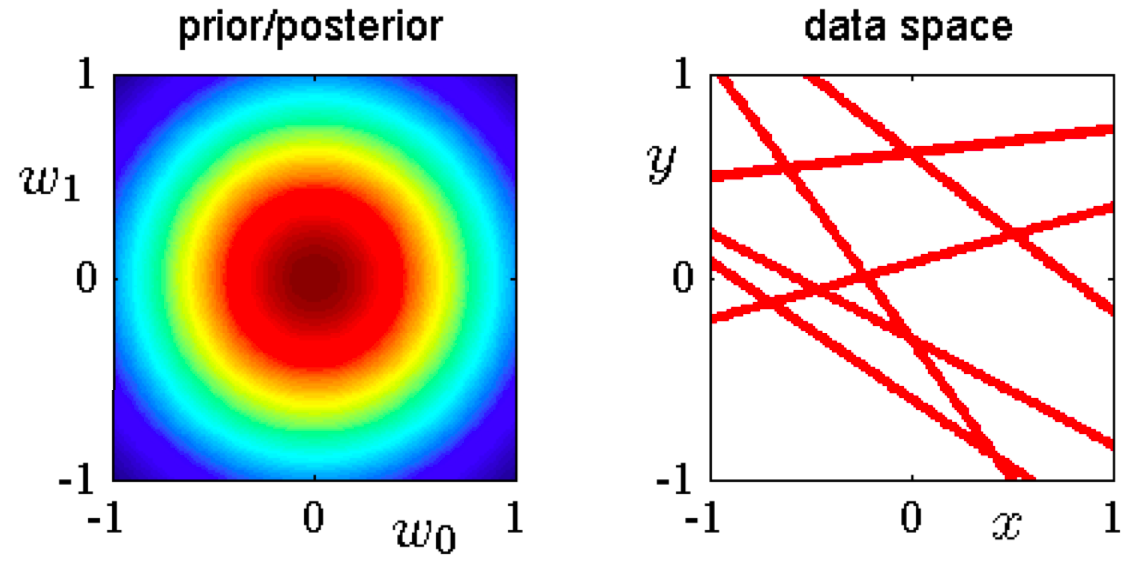
\includegraphics[width=0.6\textwidth]{figs/lin-regression-prior-PRMLFig3-7}
\par\end{center}

\begin{itemize}
\item On right,  $y(x)=\ex\left[y\mid x,w\right]=w_{0}+w_{1}x$, for randomly
chosen $w\sim p(w)=\cn\left(0,\frac{1}{2}I\right)$. 
\end{itemize}
\let\thefootnote\relax\footnotetext{\tiny{Bishop's PRML Fig 3.7}}
\end{frame}


\begin{frame}{Example in 1-Dimension: 1 Observation}
\begin{center}
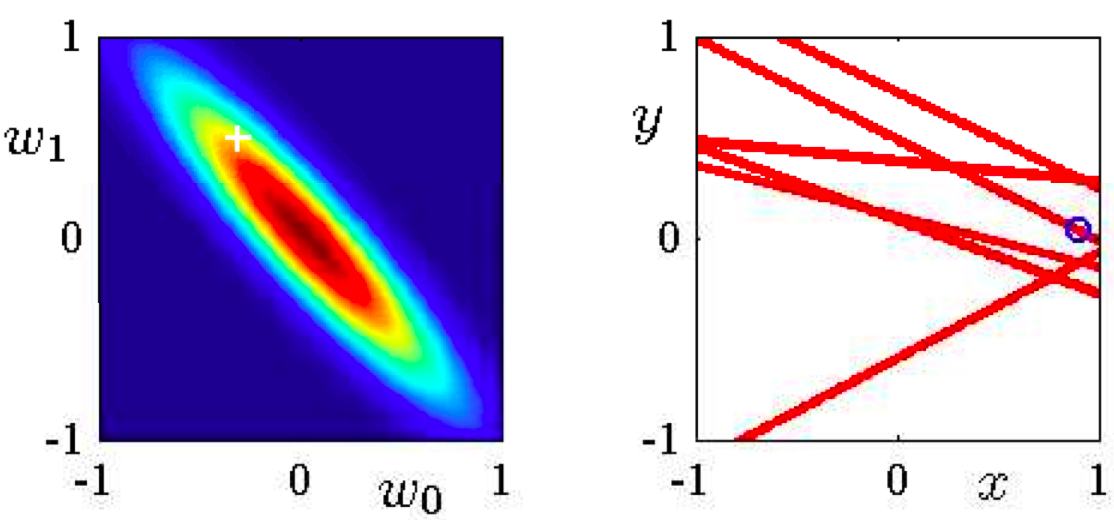
\includegraphics[width=0.6\textwidth]{{figs/lin-regression-prior-PRMLFig3-7.1pt}.png}
\par\end{center}
\begin{itemize}
\item On left: posterior distribution; white cross indicates true parameters
\item On right: 
\begin{itemize}
  \item blue circle indicates the training observation
  \item red lines,  $y(x)=\ex\left[y\mid x,w\right]=w_{0}+w_{1}x$, for randomly
  chosen $w\sim p(w | \cd )$ (posterior)
\end{itemize}
\end{itemize}

\let\thefootnote\relax\footnotetext{\tiny{Bishop's PRML Fig 3.7}}
\end{frame}
%
\begin{frame}{Example in 1-Dimension: 2 and 20 Observations}
\begin{center}
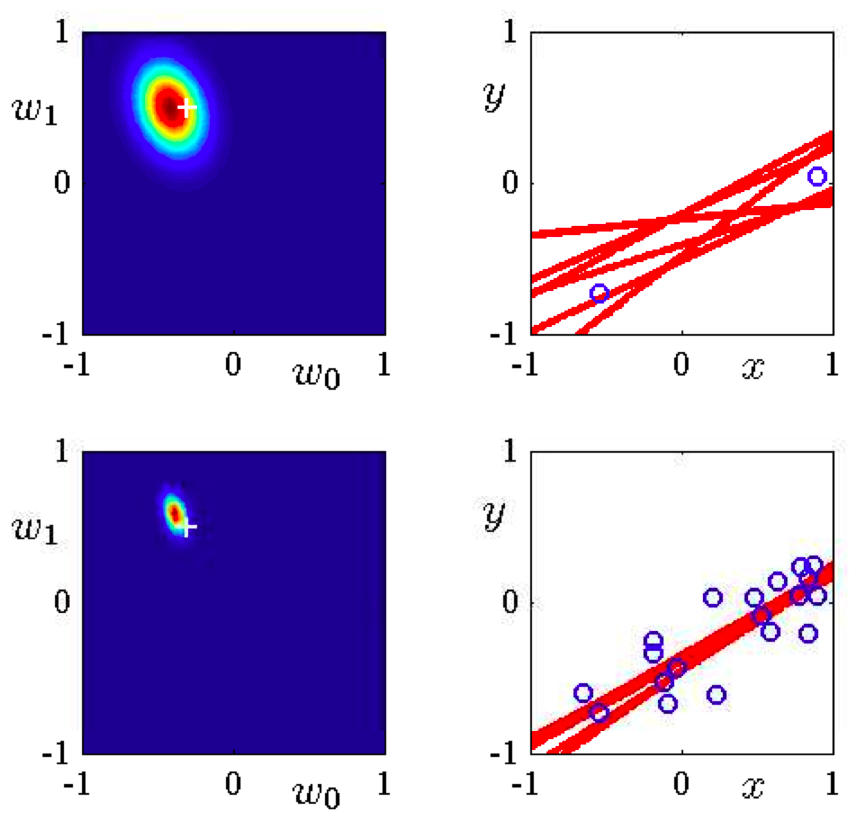
\includegraphics[height=0.7\textheight]{{figs/lin-regression-prior-PRMLFig3-7.2and20pt}.png}
\par\end{center}

\let\thefootnote\relax\footnotetext{\tiny{Bishop's PRML Fig 3.7}}
\end{frame}
%

\section{Gaussian Regression: Closed form}
\begin{frame}{Closed Form for Posterior}
\begin{itemize}
\item Model:
\begin{eqnarray*}
w & \sim & \cn\left(0,\Sigma_{0}\right)\\
\pause y_{i}\mid x,w & \text{i.i.d.} & \cn(w^{T}x_{i},\sigma^{2})
\end{eqnarray*}


\pause{}
\item Design matrix $X$ $\qquad$Response column vector $y$

\pause{}
\item \textbf{Posterior distribution is a Gaussian distribution:
\begin{eqnarray*}
w\mid\cd & \sim & \pause\cn(\mu_{P},\Sigma_{P})\\
\mu_{\text{P}} & = & \left(X^{T}X+\sigma^{2}\Sigma_{0}^{-1}\right)^{-1}X^{T}y\\
\Sigma_{\text{P}} & = & \left(\sigma^{-2}X^{T}X+\Sigma_{0}^{-1}\right)^{-1}
\end{eqnarray*}
}

\pause{}
\item \textbf{Posterior Variance} $\Sigma_{P}$ gives us a natural \textbf{uncertainty
measure.}
\end{itemize}

\end{frame}
%
\begin{frame}{Closed Form for Posterior}
\begin{itemize}
\item \textbf{Posterior distribution is a Gaussian distribution:
\begin{eqnarray*}
w\mid\cd & \sim & \pause\cn(\mu_{P},\Sigma_{P})\\
\mu_{\text{P}} & = & \left(X^{T}X+\sigma^{2}\Sigma_{0}^{-1}\right)^{-1}X^{T}y\\
\Sigma_{\text{P}} & = & \left(\sigma^{-2}X^{T}X+\Sigma_{0}^{-1}\right)^{-1}
\end{eqnarray*}
}

\pause{}
\item If we want point estimates of $w$\textbf{, MAP estimator} and the
\textbf{posterior mean} are given by
\[
\pause\hat{w}=\mu_{P}=\left(X^{T}X+\sigma^{2}\Sigma_{0}^{-1}\right)^{-1}X^{T}y
\]
 

\pause{}
\item For the prior variance $\Sigma_{0}=\frac{\sigma^{2}}{\lambda}I$,
we get
\[
\hat{w}=\mu_{P}=\left(X^{T}X+\lambda I\right)^{-1}X^{T}y,\pause
\]
which is of course the ridge regression solution. 
\end{itemize}
\end{frame}
%
\begin{comment}
\begin{frame}{Connection the MAP to Ridge Regression}
\begin{itemize}
\item The \textbf{Posterior density }on $w$\textbf{ }for\textbf{ }$\Sigma_{0}=\frac{\sigma^{2}}{\lambda}I$:\textbf{
\begin{eqnarray*}
p(w\mid\cd) & \propto & \underbrace{\exp\left(-\frac{\lambda}{2\sigma^{2}}\|w\|^{2}\right)}_{\text{prior}}\underbrace{\prod_{i=1}^{n}\exp\left(-\frac{(y_{i}-w^{T}x_{i})^{2}}{2\sigma^{2}}\right)}_{\text{likelihood}}
\end{eqnarray*}
}

\pause{}
\item To find the \textbf{MAP}, we minimize the negative log posterior:
\begin{eqnarray*}
\hat{w}_{\text{MAP}} & = & \argmin_{w\in\reals^{d}}\left[-\log p(w\mid\cd)\right]\\
\pause & = & \argmin_{w\in\reals^{d}}\underbrace{\sum_{i=1}^{n}(y_{i}-w^{T}x_{i})^{2}}_{\text{log-likelihood}}+\underbrace{\lambda\|w\|^{2}}_{\text{log-prior}}
\end{eqnarray*}


\pause{}
\item Which is the ridge regression objective.
\end{itemize}
\end{frame}
%
\begin{frame}{Predictive Posterior Distribution}
\begin{itemize}
\item Given a new input point $x_{\text{new}}$, how do we predict $y_{\text{new}}$
?

\pause{}
\item \textbf{Predictive distribution
\begin{eqnarray*}
p(y_{\text{new}}\mid x_{\text{new}},\cd) & = & \pause\int p(y_{\text{new}}\mid x_{\text{new}},w,\cd)p(w\mid\cd)\,dw\\
\pause & = & \int p(y_{\text{new}}\mid x_{\text{new}},w)p(w\mid\cd)\,dw
\end{eqnarray*}
}

\pause{}
\item For Gaussian regression, predictive distribution has closed form.
\end{itemize}
\end{frame}
%
\begin{frame}{Closed Form for Predictive Distribution}
\begin{itemize}
\item \textbf{Model}:
\begin{eqnarray*}
w & \sim & \cn\left(0,\Sigma_{0}\right)\\
\pause y_{i}\mid x,w & \text{i.i.d.} & \cn(w^{T}x_{i},\sigma^{2})
\end{eqnarray*}


\pause{ }
\item \textbf{Predictive Distribution}
\begin{eqnarray*}
p(y_{\text{new}}\mid x_{\text{new}},\cd) & = & \int p(y_{\text{new}\text{ }}\mid x_{\text{new}},w)p(w\mid\cd)\,dw.
\end{eqnarray*}

\begin{itemize}
\item Averages over prediction for each $w$, weighted by posterior distribution.

\pause{ }
\end{itemize}
\item \textbf{Closed form:}
\begin{eqnarray*}
y_{\text{new}}\mid x_{\text{new}},\cd & \sim & \cn\left(\eta_{\text{new}}\,,\,\sigma_{\text{new}}^{2}\right)\\
\pause\eta_{\text{new}} & = & \mu_{\text{P}}^{T}x_{\text{new}}\\
\pause\sigma_{\text{new}}^{2} & = & \underbrace{x_{\text{new}}^{T}\Sigma_{\text{P}}x_{\text{new}}}_{\text{from variance in }w}+\underbrace{\sigma^{2}}_{\text{inherent variance in }y}
\end{eqnarray*}
\end{itemize}
\end{frame}
%
\begin{frame}{Bayesian Regression Provides Uncertainty Estimates}
\begin{itemize}
\item With predictive distributions, we can give mean prediction with error
bands:
\end{itemize}
\begin{center}
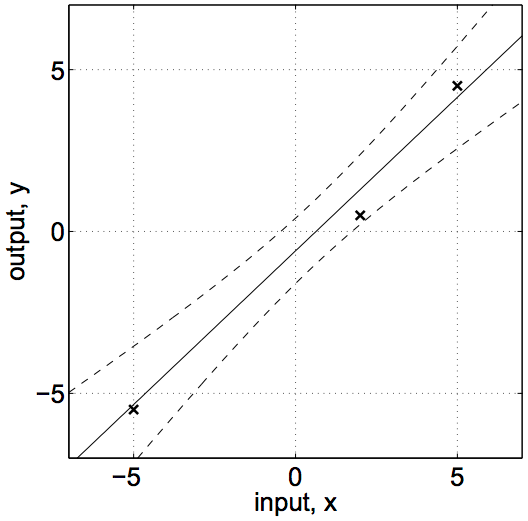
\includegraphics[height=0.7\textheight]{figs/predictiveDistWithErrorBands}
\par\end{center}

\let\thefootnote\relax\footnotetext{\tiny{Rasmussen and Williams' \emph{Gaussian Processes for Machine Learning}, Fig.2.1(b) }}
\end{frame}
\end{comment}

\end{document}

